\documentclass[10pt]{article}
\usepackage[margin=1.85cm]{geometry}
\usepackage{graphicx,booktabs,xcolor,titlesec,enumitem,amsmath,array}
\usepackage[hidelinks]{hyperref}
\definecolor{ink}{HTML}{1F2430}
\definecolor{muted}{HTML}{667085}
\definecolor{blue}{HTML}{355C7D}
\definecolor{teal}{HTML}{2A9D8F}
\definecolor{coral}{HTML}{E76F51}
\titleformat{\section}{\large\bfseries\color{ink}}{\thesection}{0.6em}{}
\titleformat{\subsection}{\normalsize\bfseries\color{ink}}{\thesubsection}{0.6em}{}
\setlist{nosep,leftmargin=1.25em}
\setlength{\parindent}{0pt}
\setlength{\parskip}{0.42em}
\newcolumntype{L}[1]{>{\raggedright\arraybackslash}p{#1}}
\newcommand{\eid}[1]{\newline\textcolor{muted}{\footnotesize
Evidence: \nolinkurl{#1}}}
\newcommand{\dev}{\textcolor{coral}{\textbf{development only}}}
\newcommand{\good}[1]{\textcolor{teal}{\textbf{#1}}}

\title{\vspace{-1.25em}J-space Phase 4 --- development synthesis\\
\large OLMo training trajectory and coordinate-frame validity\\[3pt]
\normalsize\textcolor{muted}{State through OLMo-3 32B base and 3.0 Think ·
2026-07-31}}
\author{}\date{}

\begin{document}
\maketitle
\vspace{-2.7em}

\noindent\textbf{Scope.} This is a living \dev{} report over known
Phase~3 banks. It localizes trajectory patterns and audits lens-frame
dependence; it cannot establish a binary lineage claim. No Phase~4
confirmatory or replication cell is licensed before PI sign-off and a
tagged preregistration freeze.

\section{Compute and provenance boundary}

Every model producer hard-failed unless CUDA was visible in the same
process, executed a finite FP16 CUDA matrix multiply before model load,
and recorded the device in its result envelope. Jobs ran on an NVIDIA
RTX PRO 6000 Blackwell Server Edition; the final grid allocated about
81.1\,GB VRAM. Model loading, generation, interventions, and scoring
never used CPU. CPU was limited to tests, hashes, statistics, figures,
and document compilation.

Phase~3 enters through the immutable
\texttt{p4-import-phase3-release-v1}. Native evidence is event-sourced;
registered artifacts are never overwritten.

\section{Prospective capability gate}

OLMo-3 32B Think produced 972 G5 rows, 324 facts, and 72 families under
prospective prefix-disjoint accepted-alias scoring.

\begin{center}\small
\begin{tabular}{lrrrrrr}
\toprule
view & overall & Bank F & Bank S & direct & composed & bridge supplied\\
\midrule
capability & .6430 & .4935 & .8972 & .6574 & .4846 & .7870\\
\bottomrule
\end{tabular}
\end{center}

The intervention cohort was fixed before outcomes by requiring both
direct and composed generation capability within a fact: 41/204
Bank-F facts and 85/120 Bank-S facts, or 126 facts / 252 items.
\eid{p4-g5-bank-olmo3-think-dev-v2}

The first attempt stopped after accent folding made \texttt{Río} and
\texttt{Rio} ambiguous. The repaired selector prefers exact spelling
before a unique normalized fallback; the partial attempt remains
preserved.

\section{OLMo-3 32B base point}

The exact pinned base revision
\texttt{c2b61dae89a1ad10e4ad5653d0e46b590902607b} produced 972 G5 rows.
Overall capability was .6101 (Bank F .4395; Bank S .9000). Requiring
both direct and composed capability fixed 23 Bank-F and 88 Bank-S
facts, or 111 facts / 222 items.
\eid{p4-g5-bank-olmo3-base-dev-v1}

The seven-condition grid had maximum baseline replay drift
$6.71\times10^{-7}$ nats, zero span-safe selected/protected overlap,
100\% matched-rank agreement, and maximum energy relative error
0.000260.
\eid{p4-lineage-grid-olmo3-base-dev-v1}

\begin{center}
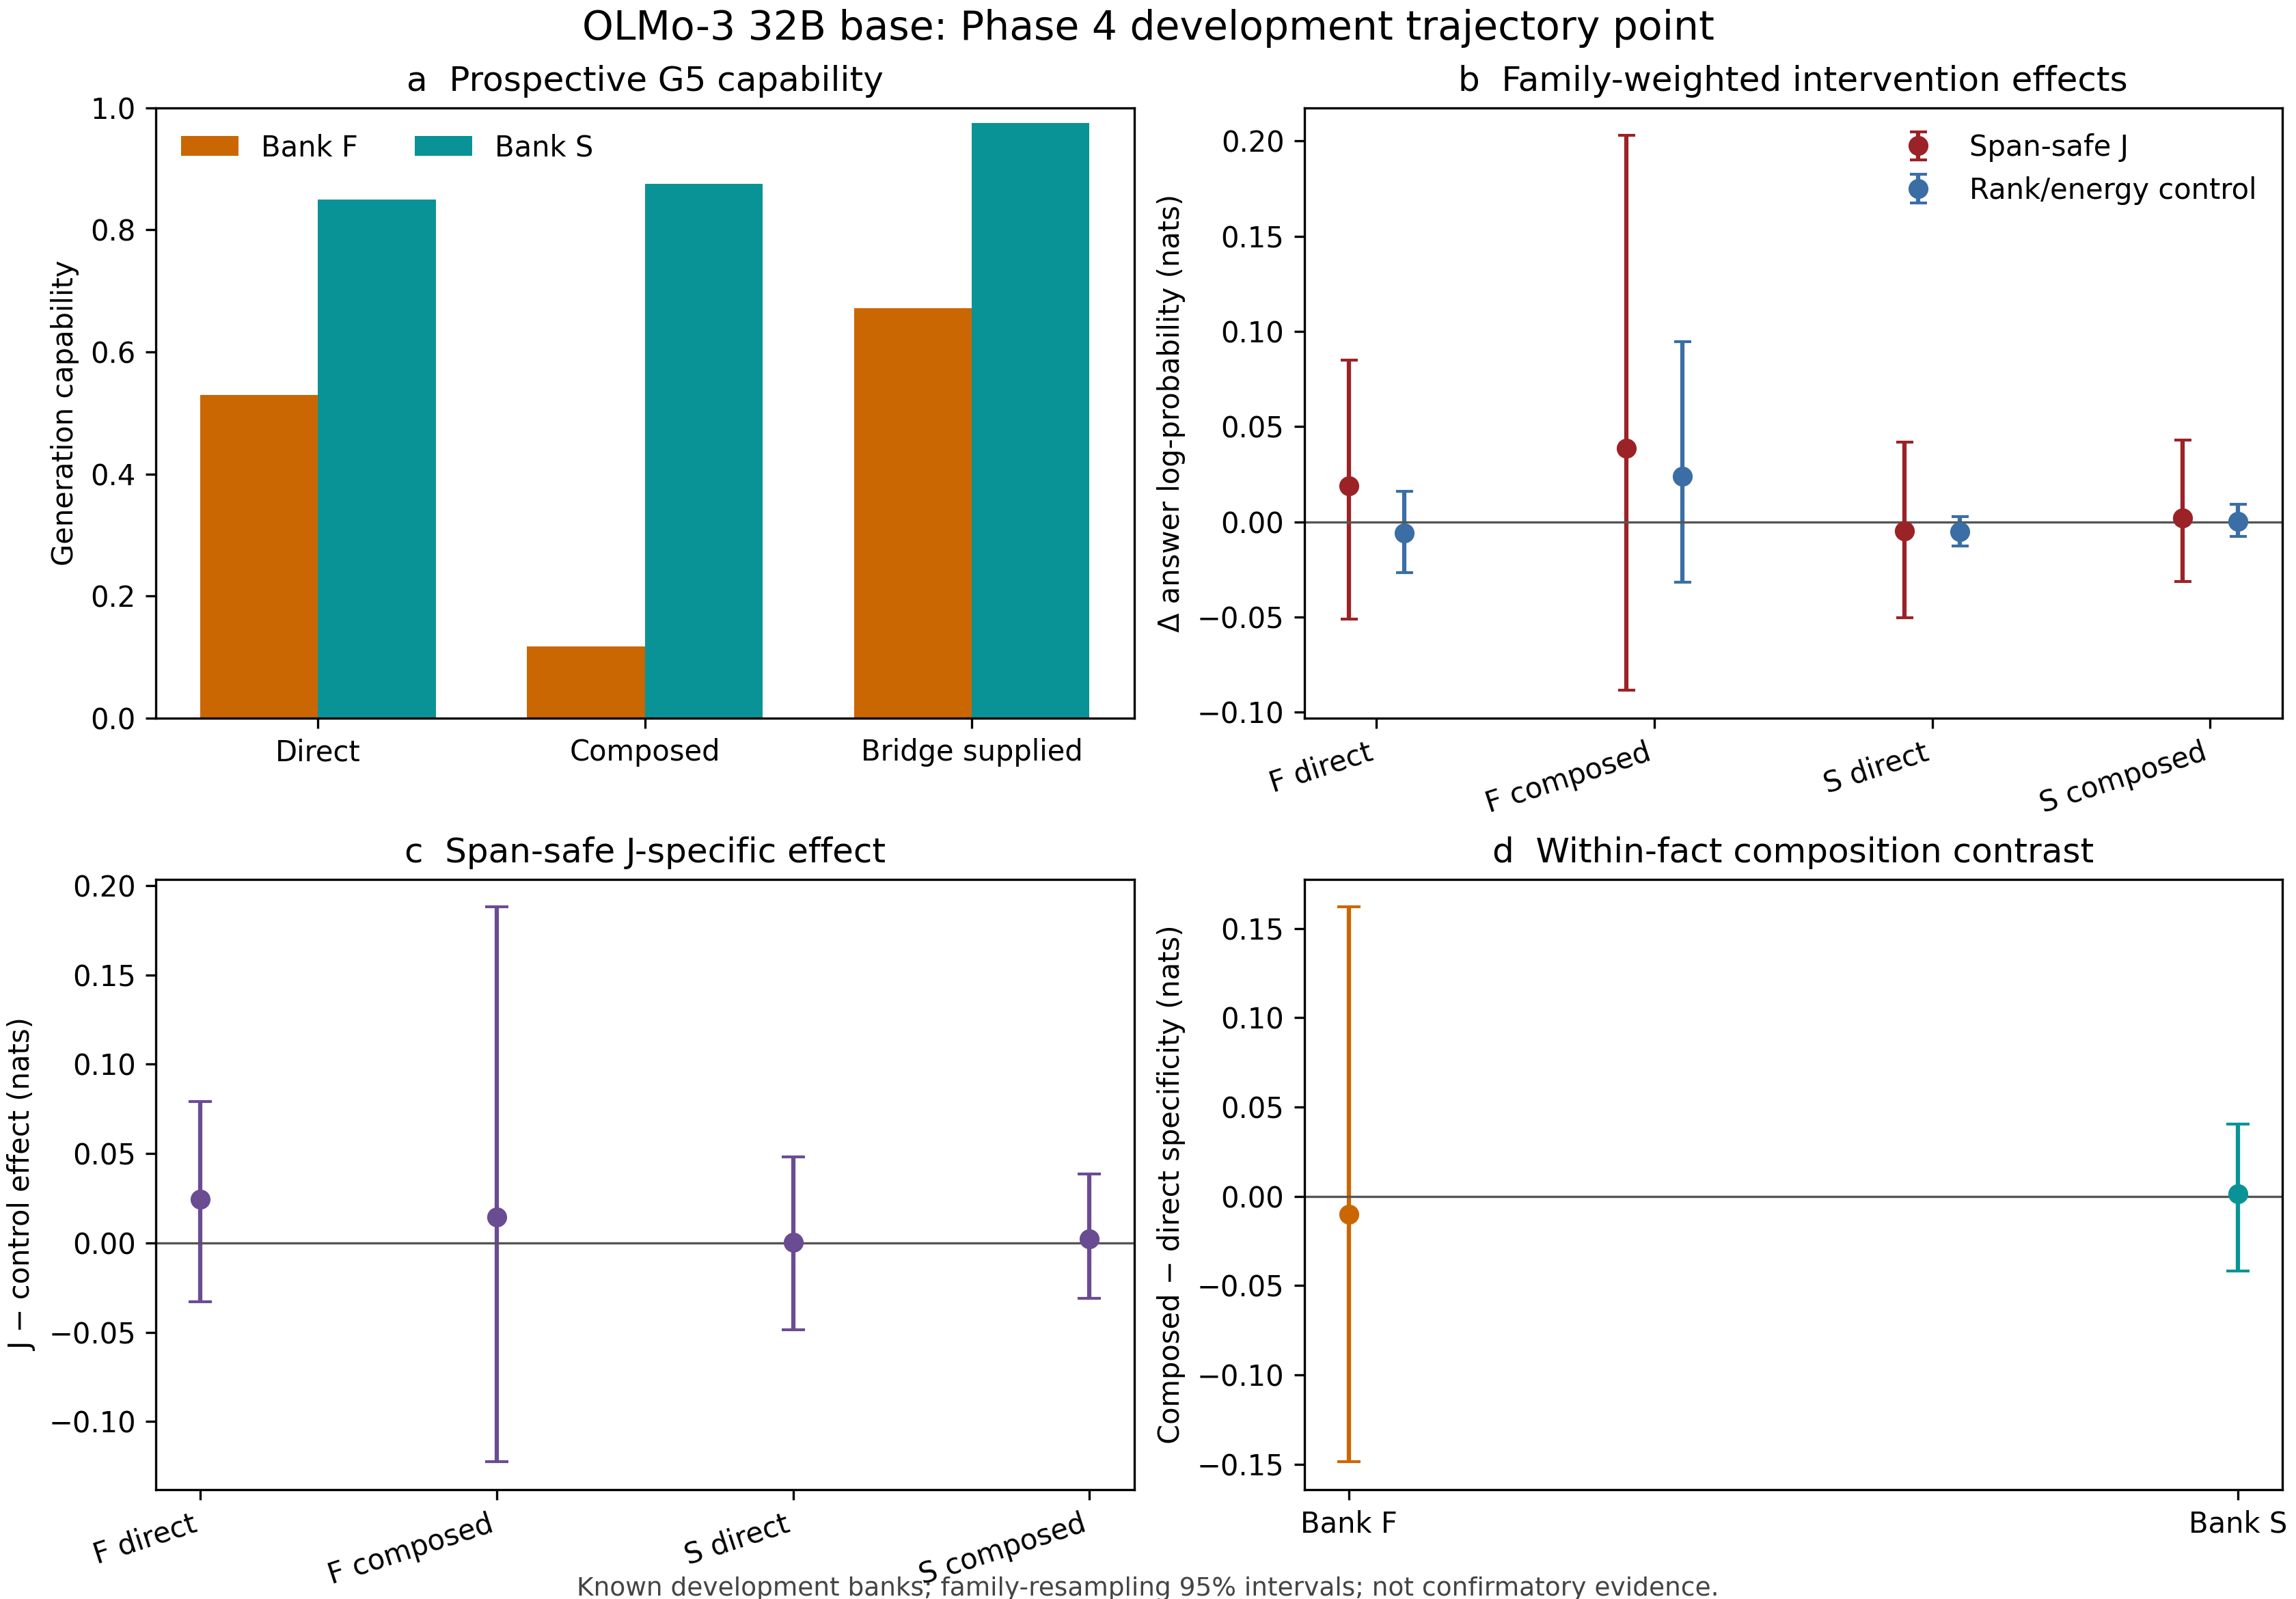
\includegraphics[width=0.82\textwidth]{../figures/p4f03_olmo3_base_development.png}
\end{center}

\begin{center}\small
\begin{tabular}{lrr}
\toprule
cell & J-specific estimate (nats) & family-bootstrap 95\% interval\\
\midrule
Bank F direct & $+0.0245$ & $[-0.0330,+0.0792]$\\
Bank F composed & $+0.0145$ & $[-0.1226,+0.1881]$\\
Bank S direct & $+0.0005$ & $[-0.0487,+0.0481]$\\
Bank S composed & $+0.0021$ & $[-0.0309,+0.0385]$\\
\bottomrule
\end{tabular}
\end{center}

All four primary effects are near zero. Bank-S
composed-minus-direct is $+0.0016\,[-0.0417,+0.0403]$. The experiment
is nevertheless sensitive: overall label-protected J-specific is
$+0.1231\,[+0.0667,+0.1802]$, while mechanics-random and
logit-protected effects are $-0.1048$ and $-0.2023$, with intervals
below zero.
\eid{p4-lineage-analysis-olmo3-base-dev-v1}

\section{Think own-lens development point}

The seven-condition grid includes baseline, span-safe J, exact
rank/energy control, label-protected J, protected-energy control,
mechanics random, and logit-space label protection. Baseline replay
drift is at most $7.15\times10^{-7}$ nats. Rank agreement is 100\%,
energy relative error is at most 0.000230, and span-safe
selected/protected overlap is zero.
\eid{p4-lineage-grid-olmo3-think-dev-v1}

\begin{center}
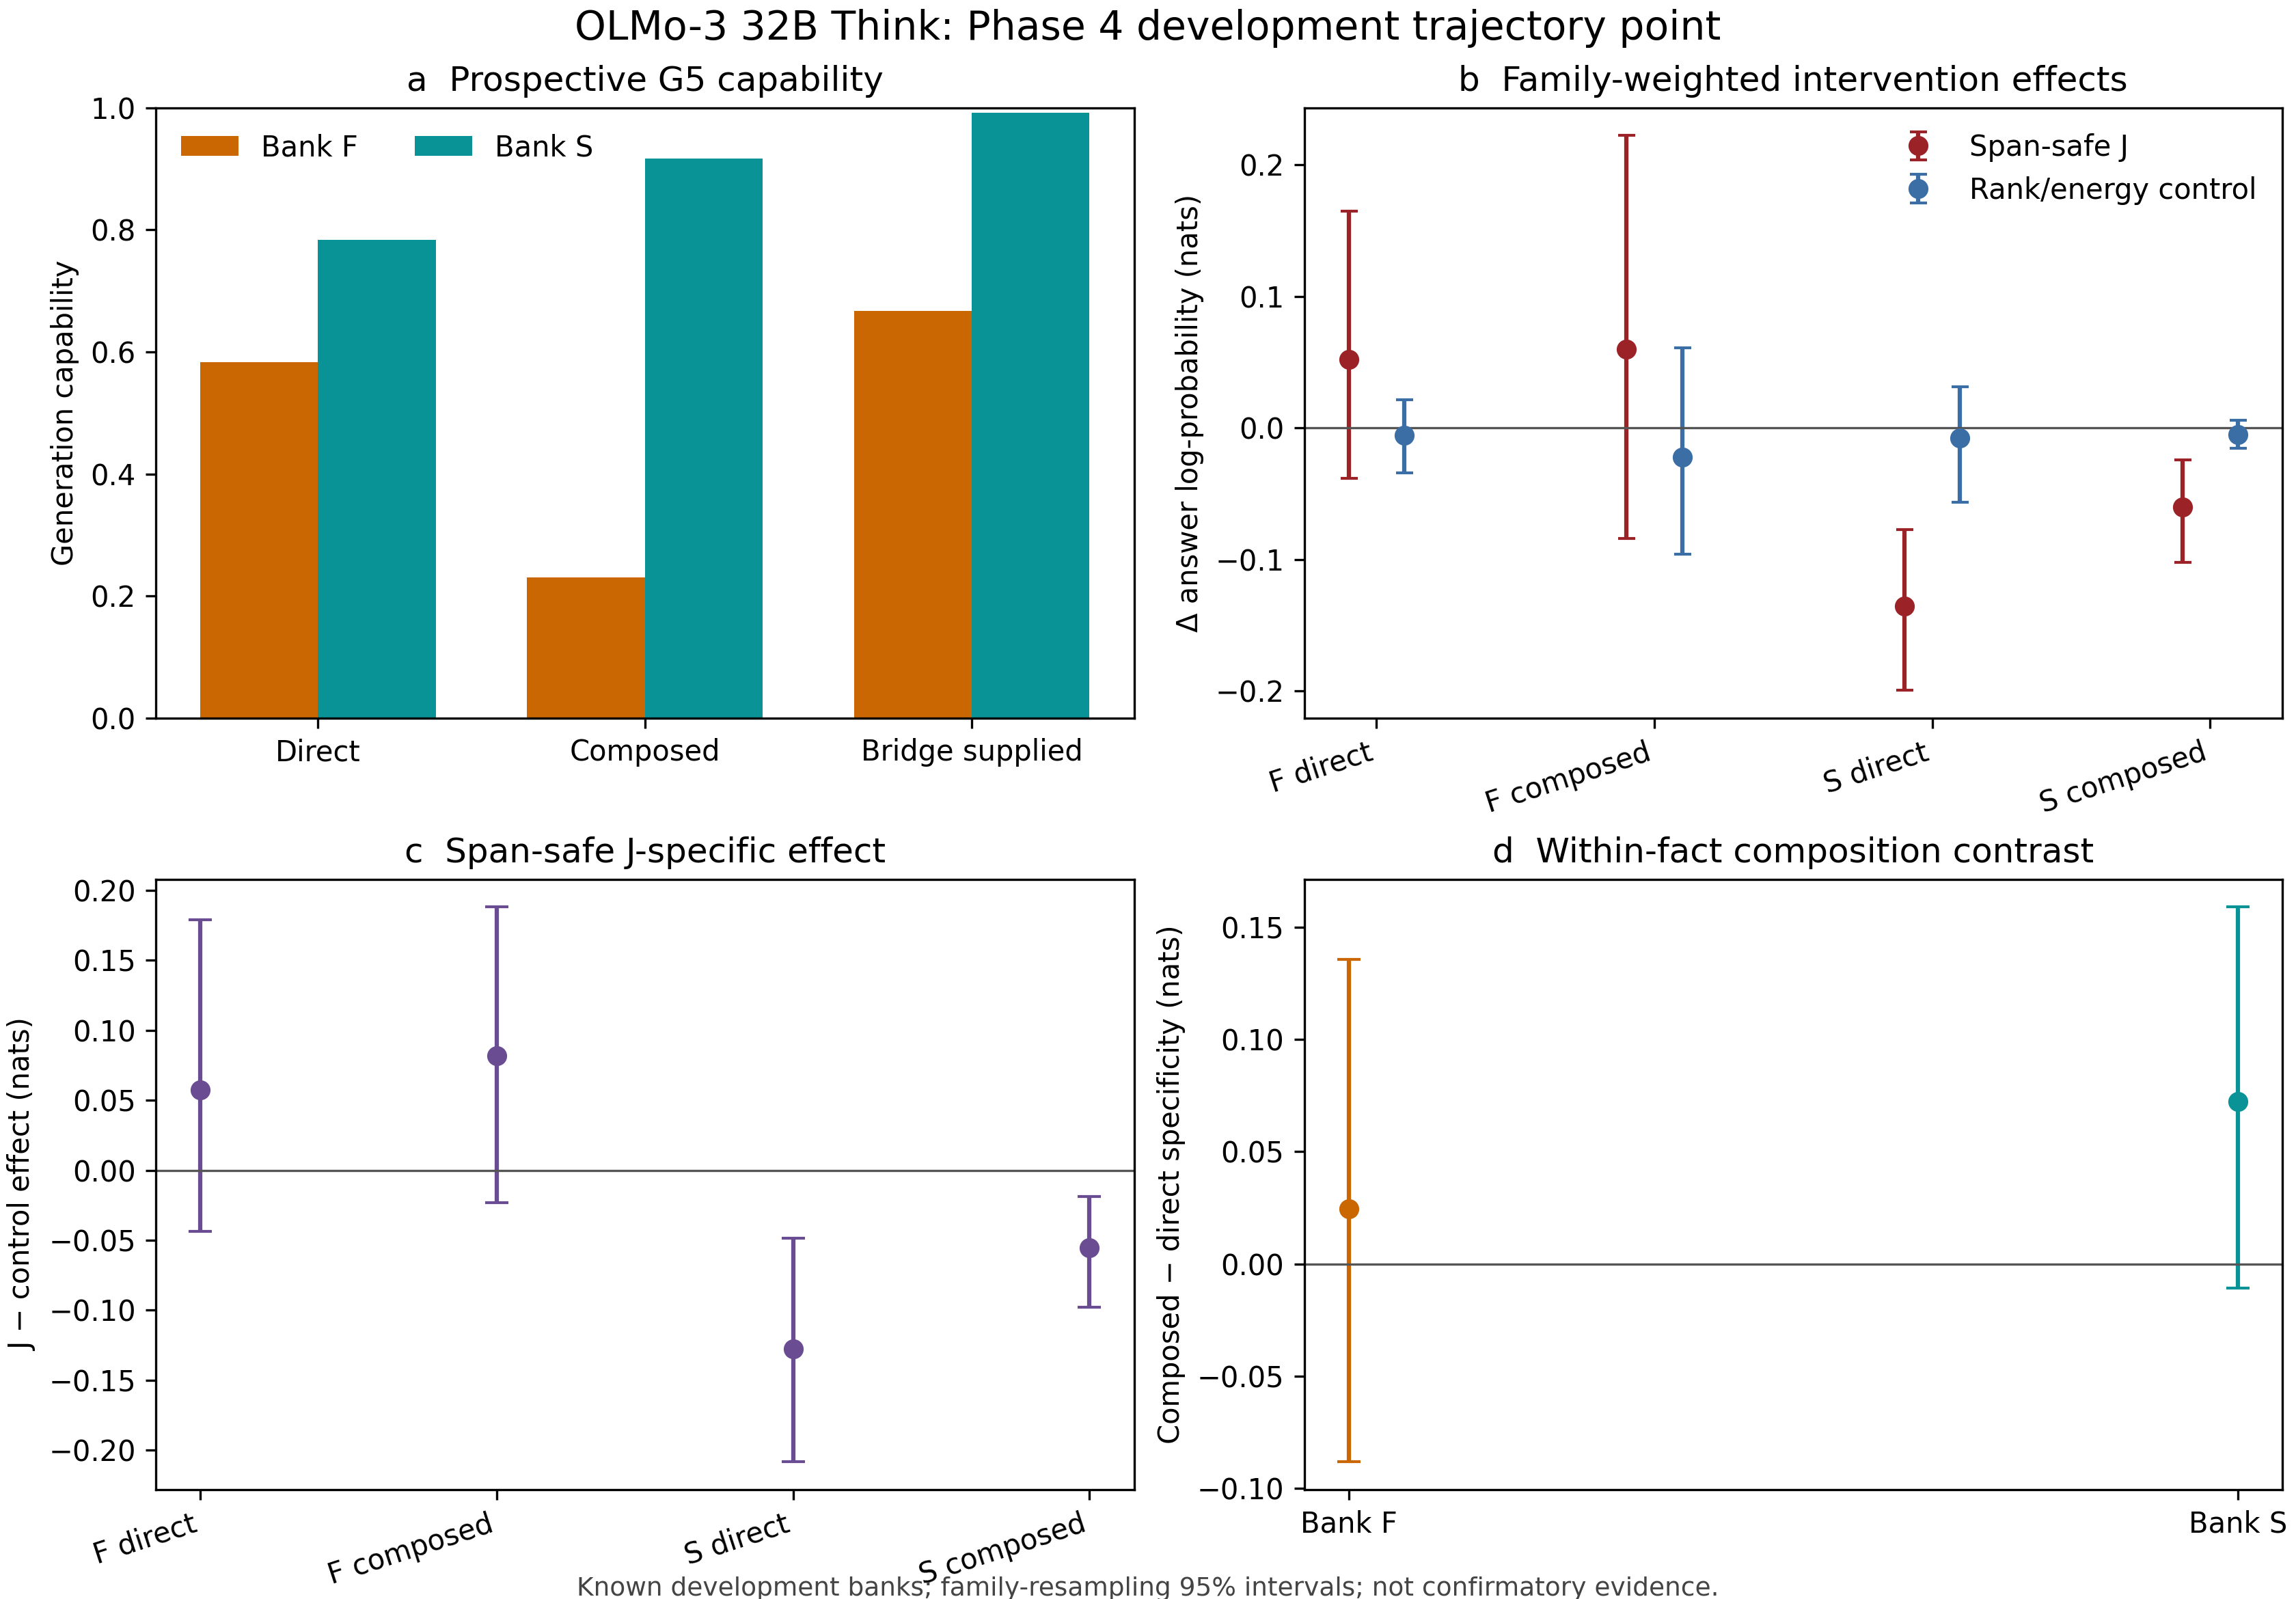
\includegraphics[width=0.95\textwidth]{../figures/p4f01_olmo3_think_development.png}
\end{center}

\begin{center}\small
\begin{tabular}{lrr}
\toprule
cell & J-specific estimate (nats) & family-bootstrap 95\% interval\\
\midrule
Bank F direct & $+0.0574$ & $[-0.0442,+0.1785]$\\
Bank F composed & $+0.0818$ & $[-0.0223,+0.1878]$\\
Bank S direct & $-0.1277$ & $[-0.2072,-0.0494]$\\
Bank S composed & $-0.0553$ & $[-0.0982,-0.0187]$\\
\bottomrule
\end{tabular}
\end{center}

Bank-S composed-minus-direct specificity is
$+0.0724\,[-0.0109,+0.1584]$. It is compatible with the unusual 3.1
Think tendency beginning by 3.0, but is not resolved and must await the
controlled Bank-W redundancy/derivation study.
\eid{p4-lineage-analysis-olmo3-think-dev-v1}

\section{Common-base-lens repair audit}

The common coordinate is the frozen OLMo base lens
(\texttt{92f32e\ldots b696}). V1 exposed rank-limited
protected-energy sites that omitted one requested component without
being marked clamped. V2 repaired the metadata but revealed that the
evidence ID itself changed all matched/random seeds.

V3 freezes the scientific-seed namespace to v1. All seven aggregate
outcome columns, every per-alias score, and every condition order match
v1 exactly (maximum difference 0). The fix reclassifies 296 summaries
and reduces the erroneous maximum unclamped energy error from 0.511283
to 0.000239 while retaining 100\% rank agreement. V3 supersedes both
withdrawn diagnostic attempts.
\eid{p4-lineage-grid-olmo3-think-common-base-lens-dev-v3}

\section{Own lens versus common base lens}

The comparison pairs all 252 items exactly; baseline drift is zero.

\begin{center}
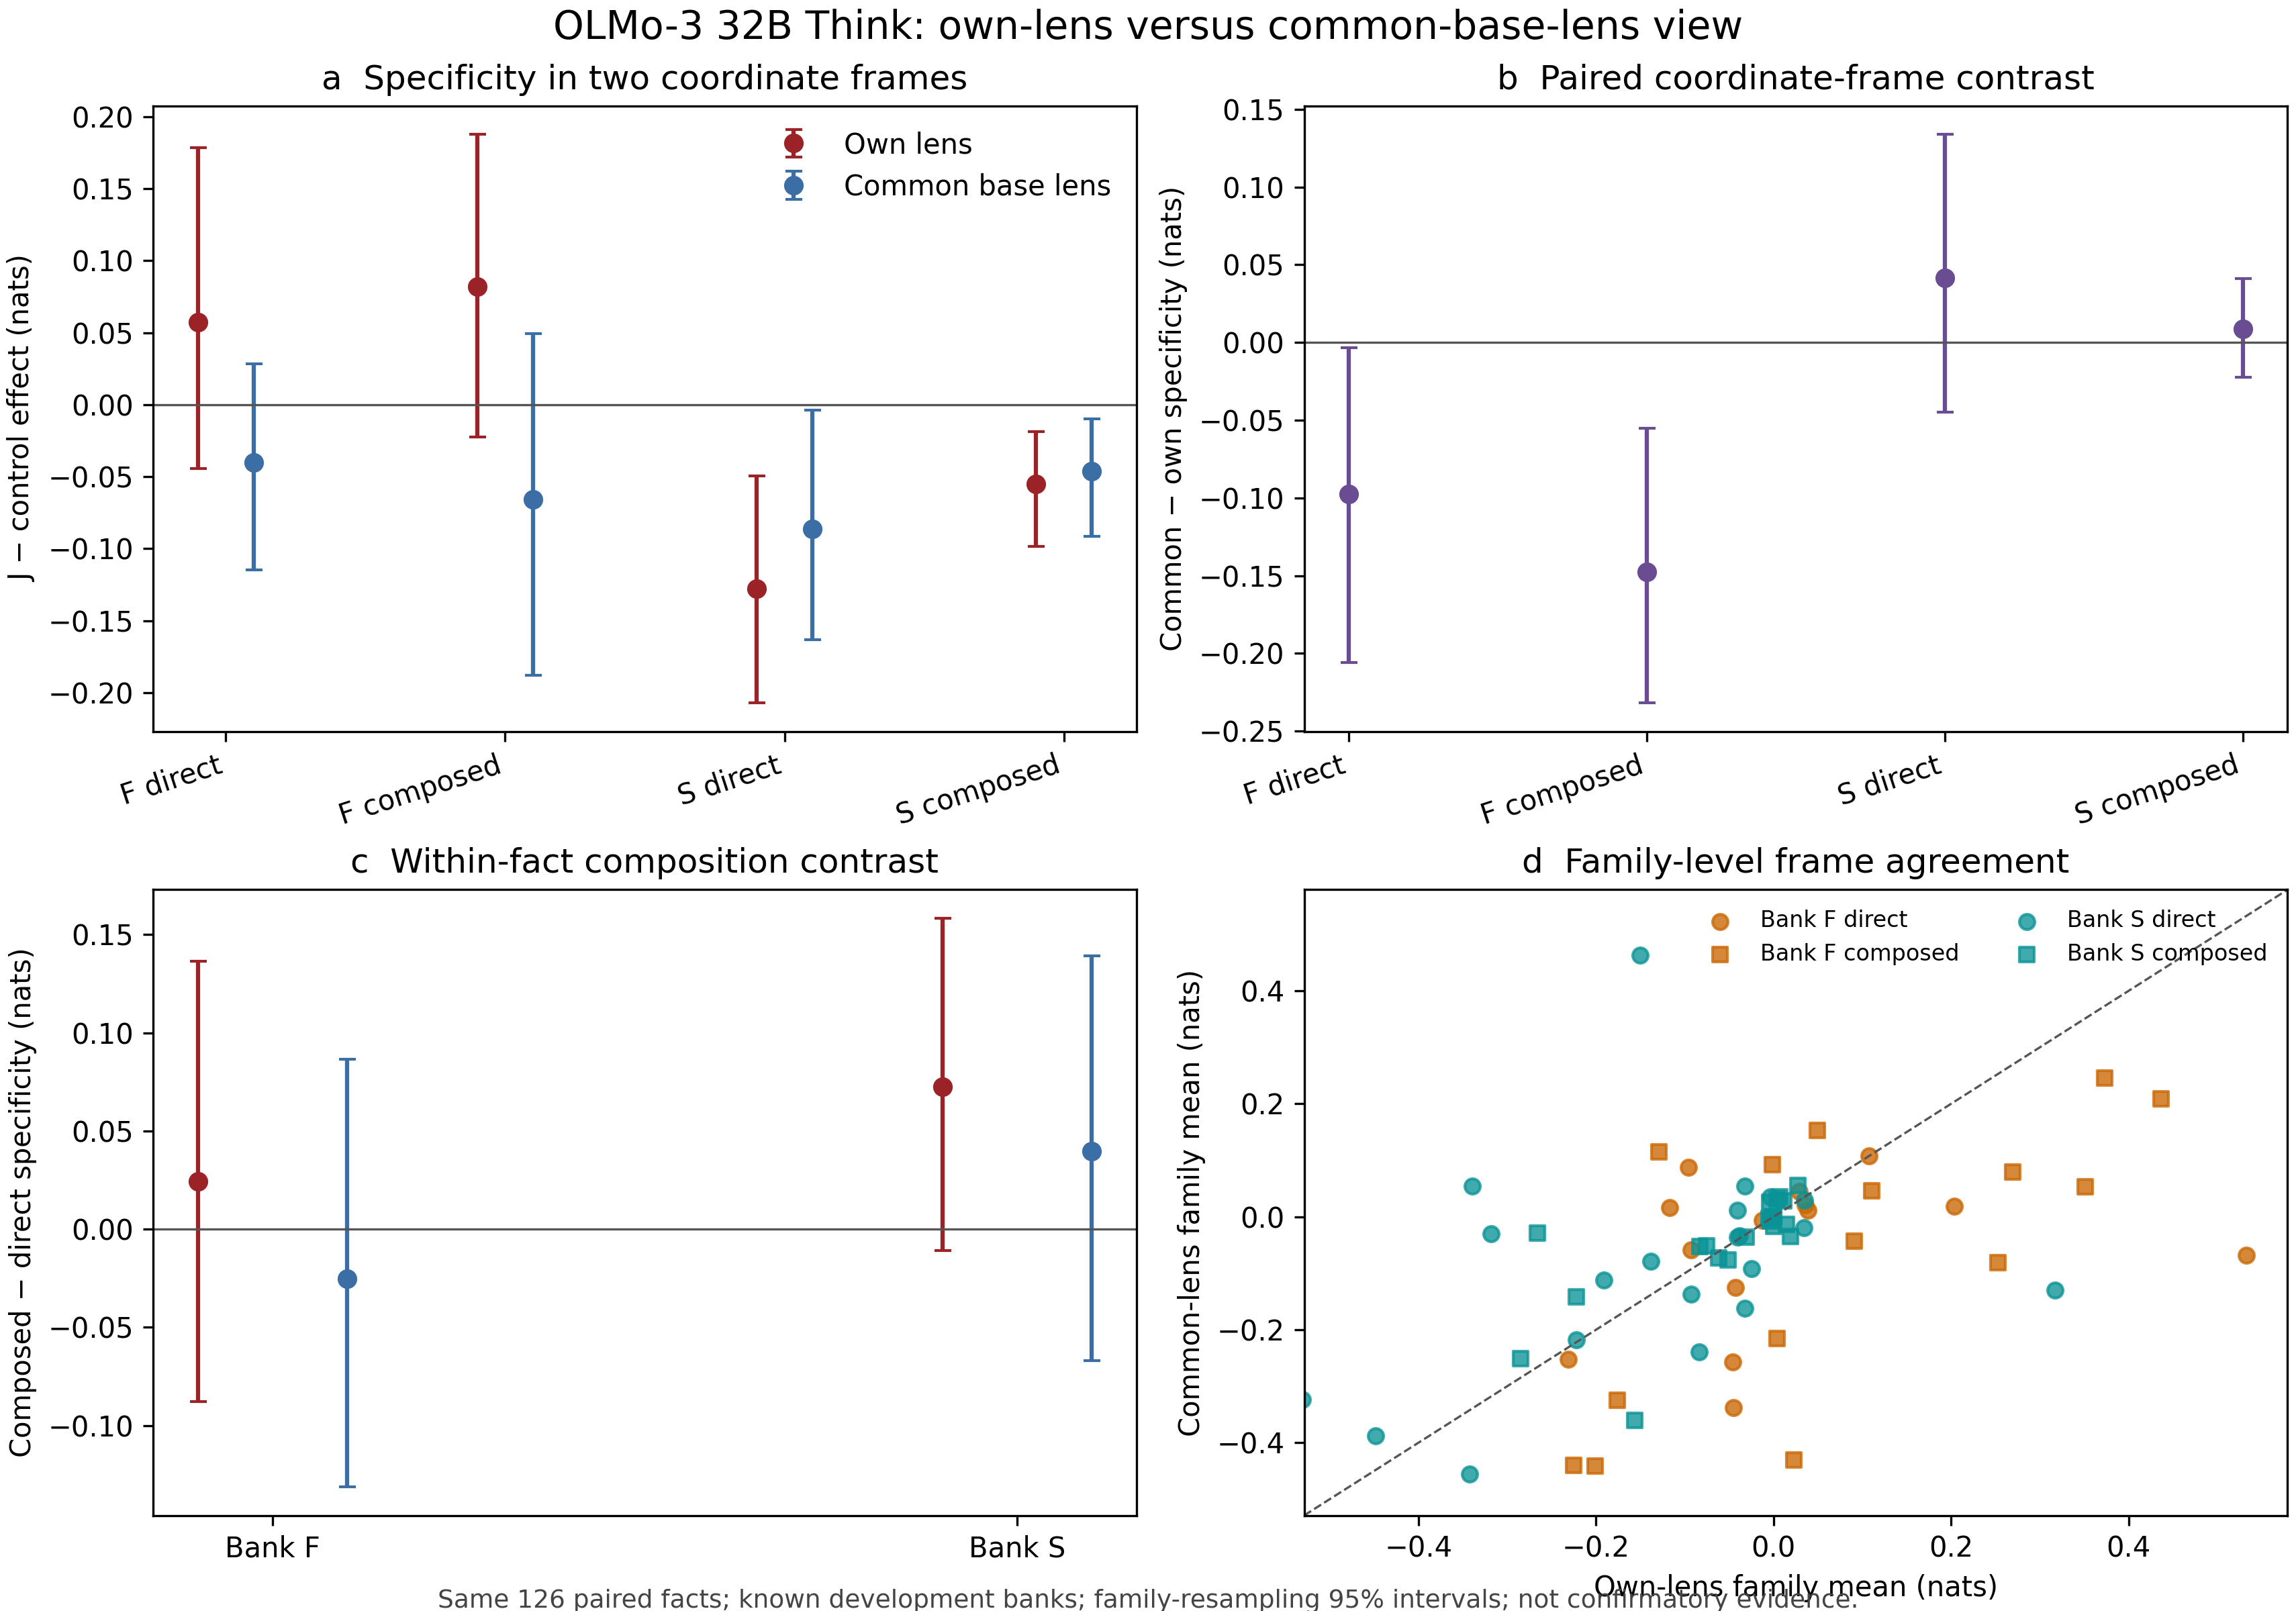
\includegraphics[width=0.80\textwidth]{../figures/p4f02_olmo3_think_lens_frame_comparison.png}
\end{center}

\begin{center}\small
\renewcommand{\arraystretch}{1.12}
\begin{tabular}{lrrr}
\toprule
cell & own lens & common base lens & common $-$ own [95\% interval]\\
\midrule
F direct & $+0.0574$ & $-0.0403$ &
$-0.0977\,[-0.2060,-0.0034]$\\
F composed & $+0.0818$ & $-0.0656$ &
$-0.1474\,[-0.2320,-0.0553]$\\
S direct & $-0.1277$ & $-0.0861$ &
$+0.0416\,[-0.0449,+0.1340]$\\
S composed & $-0.0553$ & $-0.0464$ &
$+0.0089\,[-0.0222,+0.0412]$\\
\bottomrule
\end{tabular}
\end{center}

\good{Bank S is comparatively frame-robust:} direct and composed
specificity remain negative in both views, and paired frame differences
cross zero. Bank F changes from small positive own-lens estimates to
small negative common-lens estimates; both paired frame-contrast
intervals lie below zero. Item-level own/common correlation is 0.614
and family-level correlation is 0.495.

The Bank-S composition tendency is $+0.0724$ under the own lens and
$+0.0397$ under the common lens; their difference is
$-0.0327$ with an interval crossing zero.
\eid{p4-lens-frame-analysis-olmo3-think-dev-v1}

\section{Interpretation and next boundary}

\begin{enumerate}
\item The base checkpoint is near zero in all four primary cells.
Bank-S direct and composed specificity is negative by 3.0 Think and is
comparatively stable across fitted frames.
\item Because capability cohorts are checkpoint-specific, this
localizes a base-to-Think trajectory change but is not a paired causal
estimate.
\item Bank-F conclusions depend materially on whether the checkpoint
uses its own fitted lens or the frozen base coordinate. Coordinate
drift is part of the result, not a nuisance to conceal.
\item The positive Bank-S composition tendency remains uncertain.
\item None of these known-bank estimates licenses ``lineage present''
or ``lineage absent.''
\end{enumerate}

The pinned base checkpoint is complete and banked. Next, run the exact
3.1 Think and 3.1 Instruct checkpoints through the Phase~4 prospective
G5 gate and the same seven-condition GPU grid, retaining both own-lens
and frozen common-base-lens views. Then synthesize the full base
$\rightarrow$ 3.0 Think $\rightarrow$ 3.1 Think/Instruct trajectory.
If the two coordinate views disagree, prioritize the fit-size/corpus
study before stronger causal interpretation.

\end{document}
